\documentclass[oneside, 10pt, a4]{article}
\usepackage{times}
\usepackage{graphicx}

\begin{document}

\title{Software Engineering Group Project - 7096A}
\author{Semester 1 Week 13 - Group 1}
\date{Fri Jun 13, 2008}

\maketitle

\section*{Ticket 148 - Configuring daemon through web interface}

\paragraph{} By Filimoni Lutunaika (1154924)


\subsection*{Introduction}

\paragraph{}
The earth daemon is presently only configurable through the command line. This ticket proposes the adaptation
of this configuration option onto the web-based user interface.

\subsection*{Task Description}

\paragraph{}
As the configuration methods exists on the earth daemon, this task simply involved invoking them through the controller
and presenting the configuration options on the web-based user interface.

\subsection*{Implementation}

\paragraph{}
The decision was made to create a separate daemon configuration page in order to prevent overly populating
the existing server pages and presenting the configuration options within close vicinity of each other.

\newpage


\subsection*{Results}

\paragraph{}
The following screenshot depicts the newly added configuration page of the web-based user interface.

\begin{figure}[h!]
\begin{center}
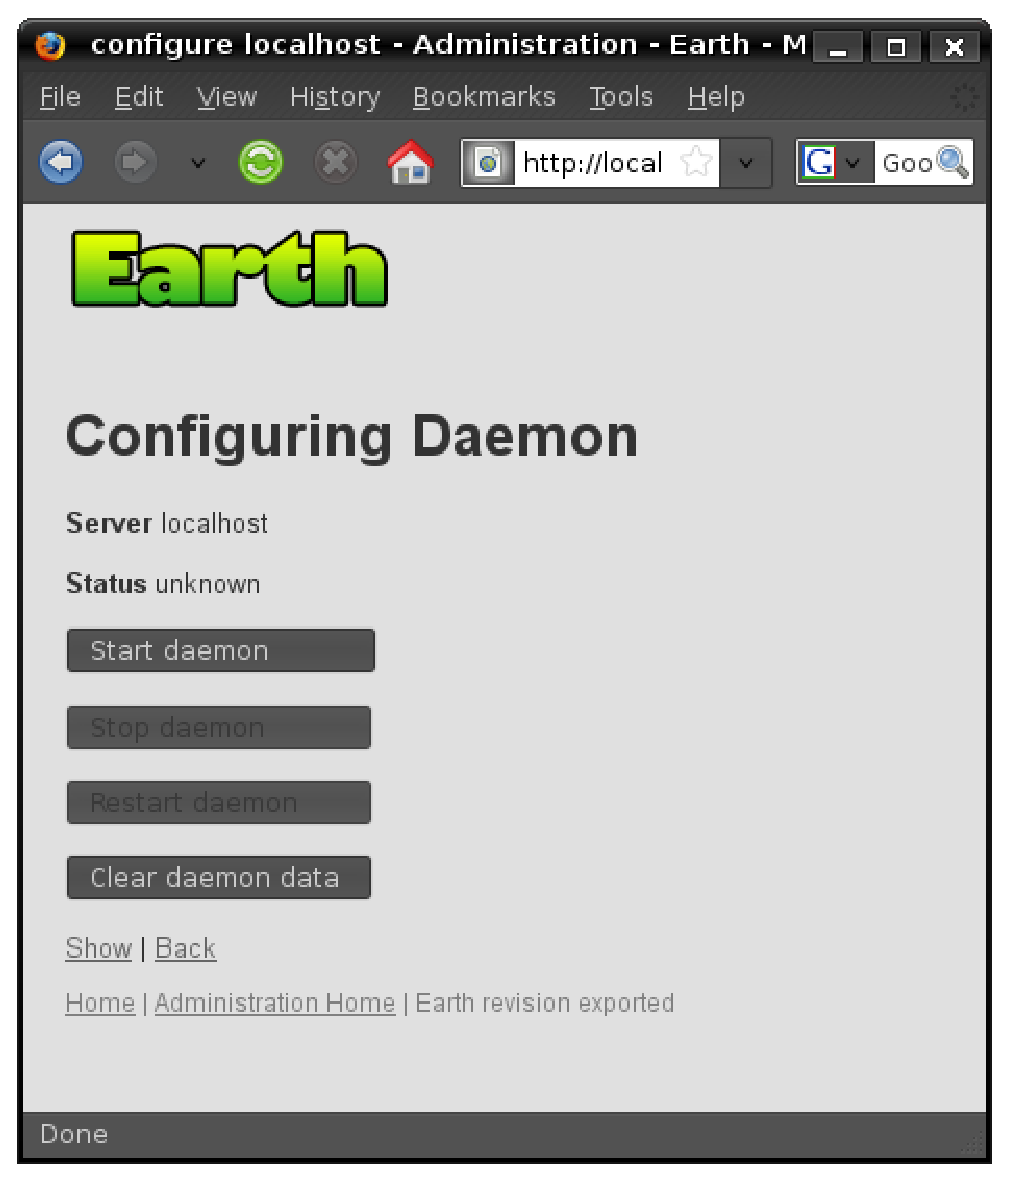
\includegraphics[width=90mm]{figs/screenshot}
\end{center}
\caption{Directory listing with delete column.}
\label{fig:screenshot}
\end{figure}

\paragraph{}
The only exception to this arrangement was the option to add directory. It was decided that this particular
option would be better placed on the server page (shown below) to ensure visual feedback to the user during
the invocation of this particular option.


\begin{figure}[h!]
\begin{center}
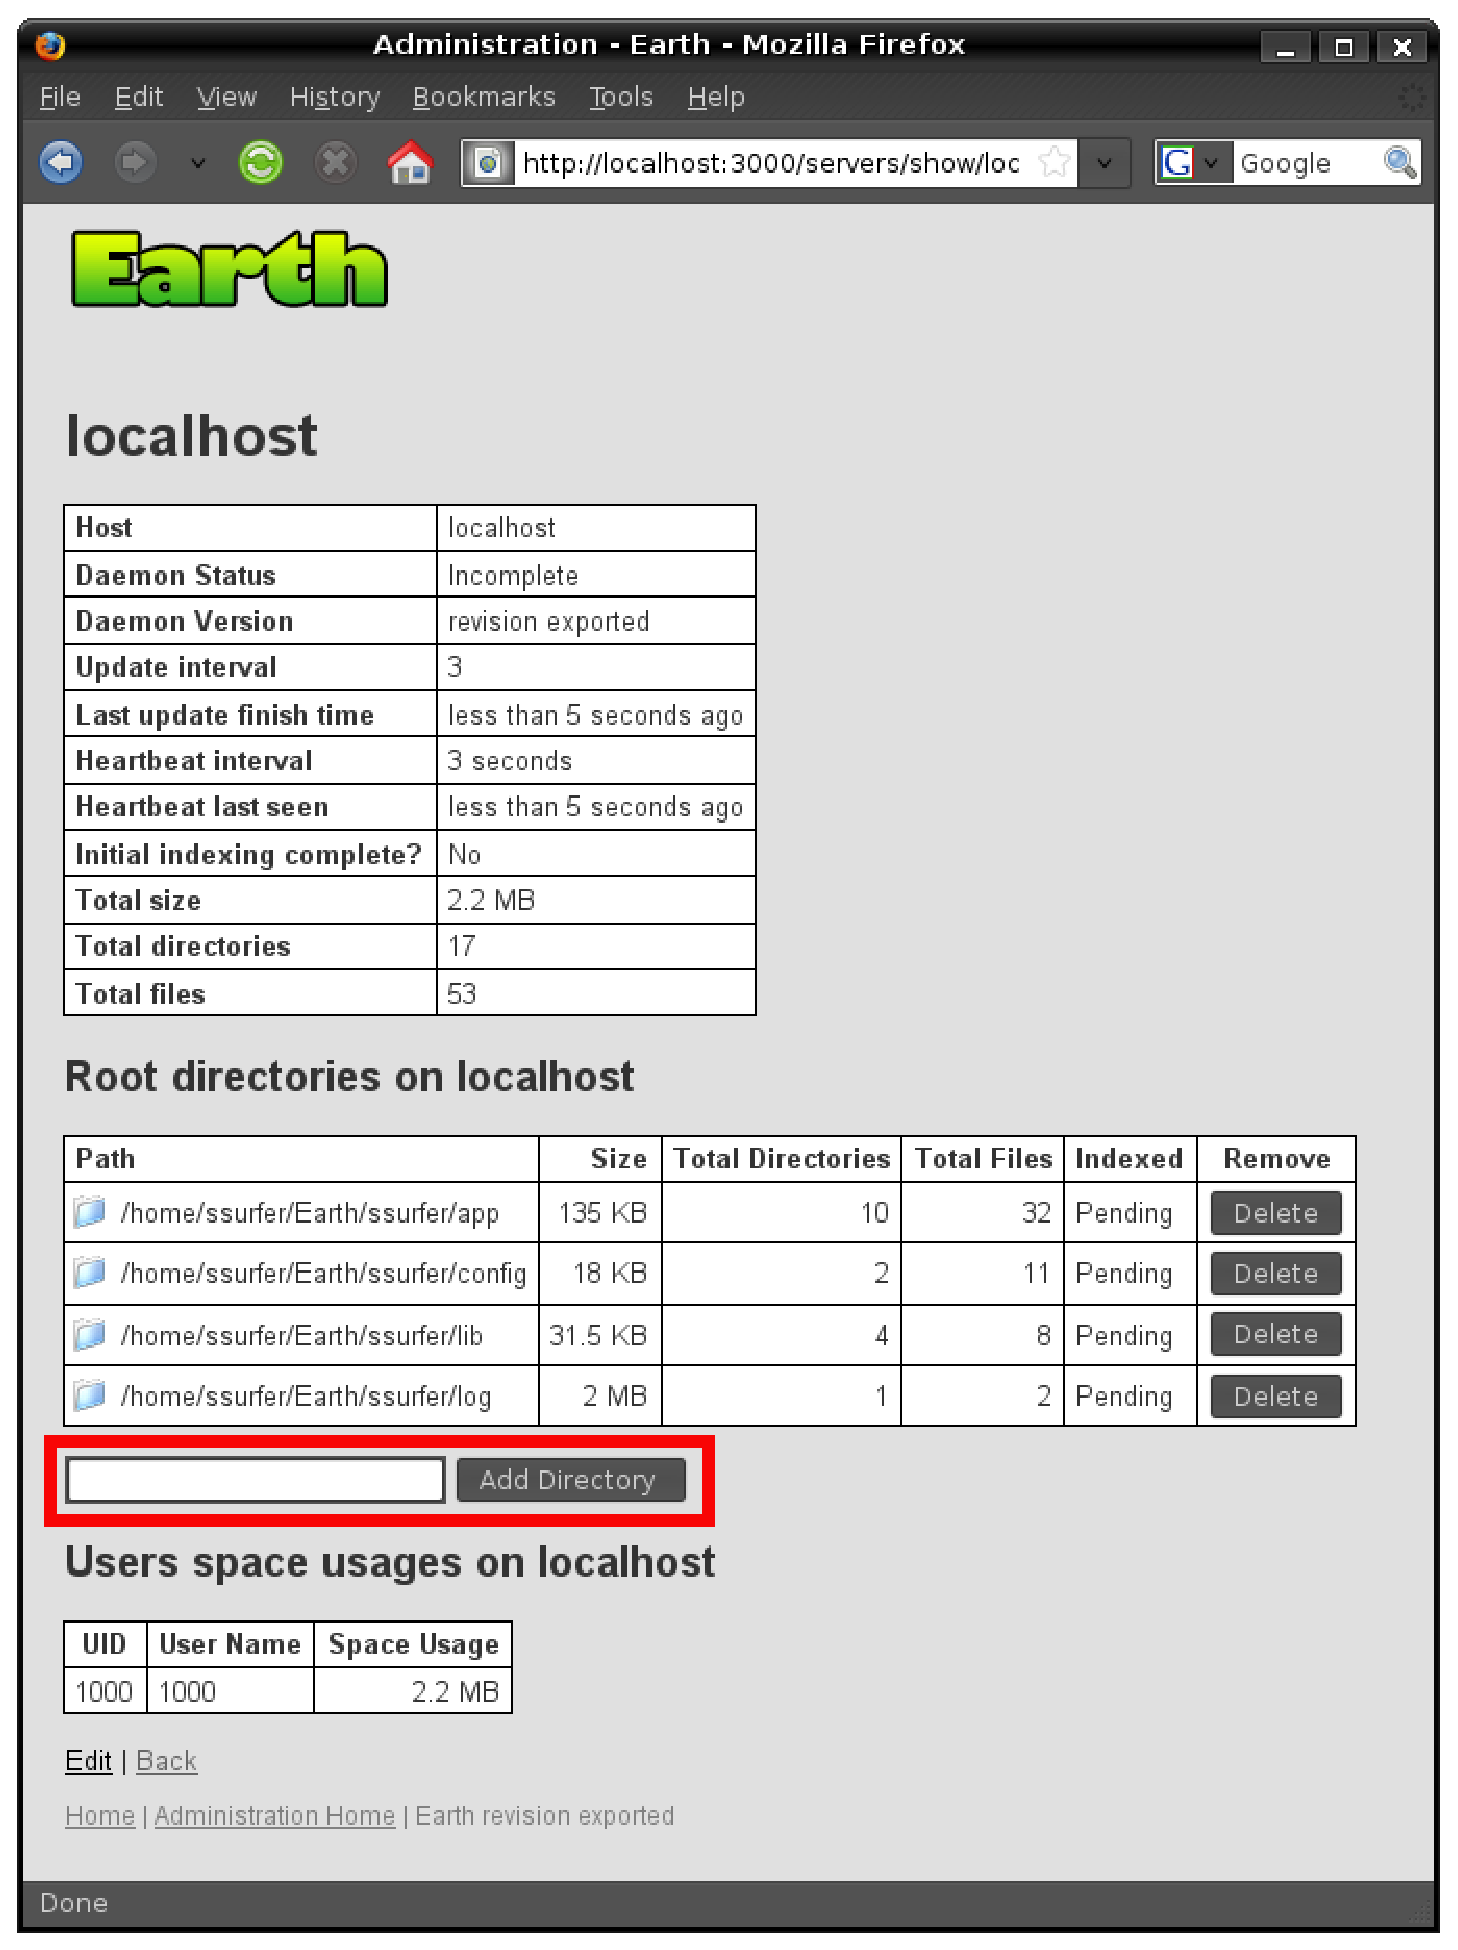
\includegraphics[width=90mm]{figs/addoption}
\end{center}
\caption{Directory listing with delete column.}
\label{fig:addoption}
\end{figure}


\paragraph{}

\subsection*{Discussion}
Presently, the add directory implementation uses a normal text box to input the name of the directory. This
might have been adequate for demonstrating the operation of the add feature through the web-based user interface.
However, a much better option would be to use a treeview option to browse the file system and select the directory.
This option would be raised in the separate ticket as a minor enhancement of the user interface.


\subsection*{Conclusion}

\paragraph{}
The daemon configuration options were successfully integrated to the web-based user interface. However, the current state
of the user interface would still require some minor enhancement before actual commissioning and deployment of the application.

\[\emph{End}\]
\end{document}
